\documentclass{standalone}
\usepackage{tikz}
\usetikzlibrary{patterns}
\usetikzlibrary{positioning}
\usetikzlibrary{patterns, positioning}
\usetikzlibrary{shapes.misc}
\usepackage[outline]{contour}
\contourlength{1.5pt} 
\usepackage[sfdefault]{ClearSans}

\begin{document}
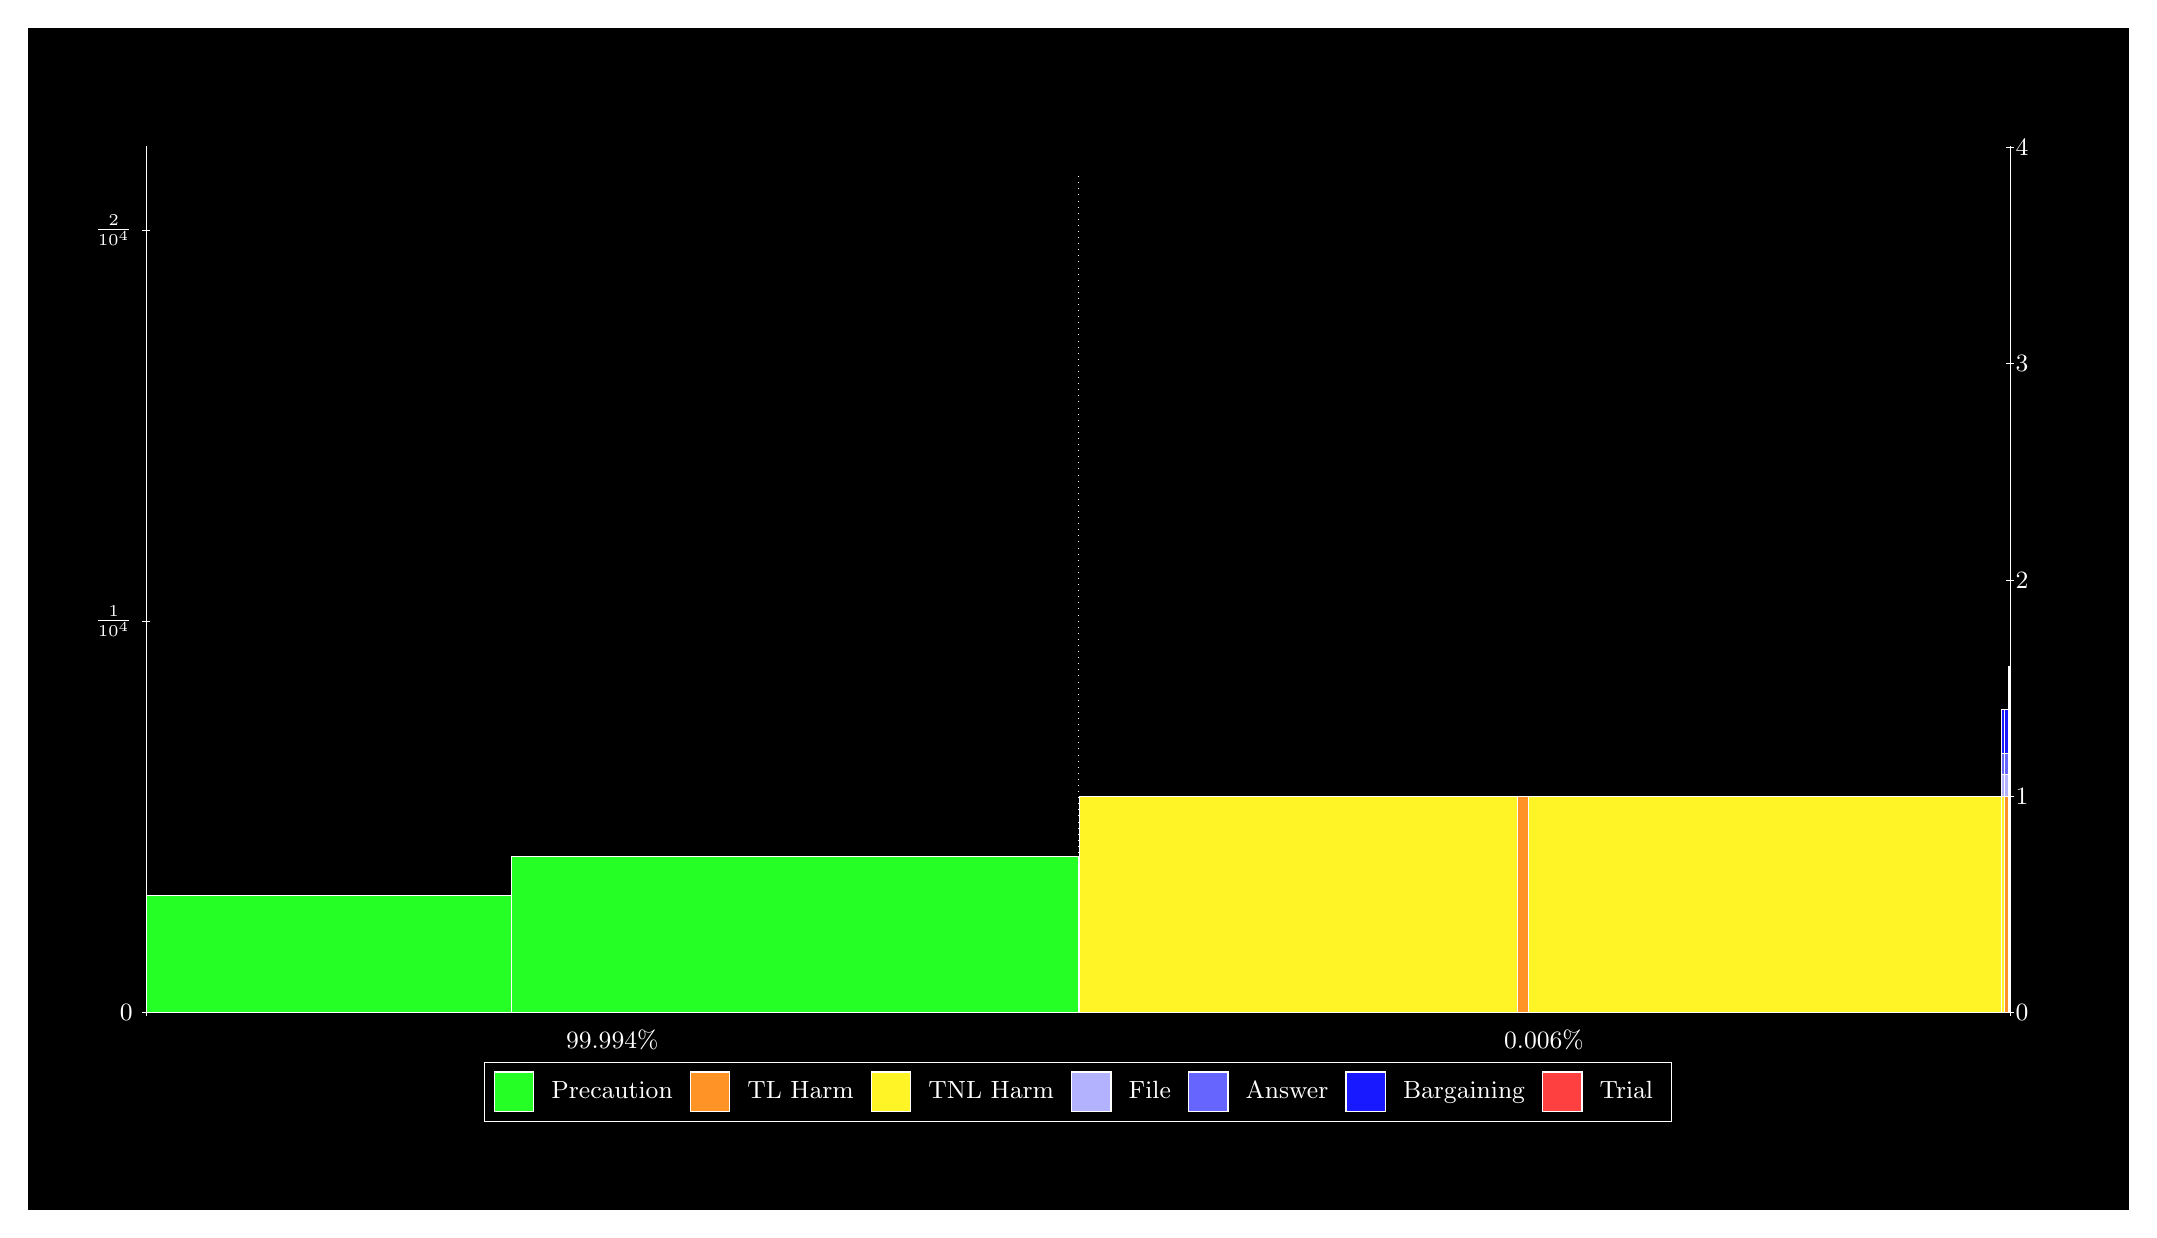
\begin{tikzpicture}
\draw[fill=black] (0,0) rectangle (26.667,15);
\draw[fill=green!85,draw=white,very thin] (1.5,2.5) rectangle (6.1371,3.9906);
\draw[fill=green!85,draw=white,very thin] (6.1371,2.5) rectangle (13.333,4.4874);
\draw[fill=green!85,draw=white,very thin] (13.333,2.5) rectangle (13.35,2.5001);
\draw[fill=blue!30,draw=white,very thin] (13.333,2.5001) rectangle (13.35,2.7747);
\draw[fill=blue!60,draw=white,very thin] (13.333,2.7747) rectangle (13.35,3.0493);
\draw[fill=blue!90,draw=white,very thin] (13.333,3.0493) rectangle (13.35,3.5986);
\draw[fill=green!85,draw=white,very thin] (13.35,2.5) rectangle (18.911,2.5001);
\draw[fill=yellow!85,draw=white,very thin] (13.35,2.5001) rectangle (18.911,5.2463);
\draw[fill=green!85,draw=white,very thin] (18.911,2.5) rectangle (19.046,2.5001);
\draw[fill=orange!85,draw=white,very thin] (18.911,2.5001) rectangle (19.046,5.2463);
\draw[fill=green!85,draw=white,very thin] (19.046,2.5) rectangle (25.053,2.5001);
\draw[fill=yellow!85,draw=white,very thin] (19.046,2.5001) rectangle (25.053,5.2464);
\draw[fill=green!85,draw=white,very thin] (25.053,2.5) rectangle (25.095,2.5001);
\draw[fill=yellow!85,draw=white,very thin] (25.053,2.5001) rectangle (25.095,5.2463);
\draw[fill=blue!30,draw=white,very thin] (25.053,5.2463) rectangle (25.095,5.521);
\draw[fill=blue!60,draw=white,very thin] (25.053,5.521) rectangle (25.095,5.7956);
\draw[fill=blue!90,draw=white,very thin] (25.053,5.7956) rectangle (25.095,6.3448);
\draw[fill=green!85,draw=white,very thin] (25.095,2.5) rectangle (25.148,2.5001);
\draw[fill=orange!85,draw=white,very thin] (25.095,2.5001) rectangle (25.148,5.2463);
\draw[fill=blue!30,draw=white,very thin] (25.095,5.2463) rectangle (25.148,5.521);
\draw[fill=blue!60,draw=white,very thin] (25.095,5.521) rectangle (25.148,5.7956);
\draw[fill=blue!90,draw=white,very thin] (25.095,5.7956) rectangle (25.148,6.3448);
\draw[fill=green!85,draw=white,very thin] (25.148,2.5) rectangle (25.162,2.5001);
\draw[fill=yellow!85,draw=white,very thin] (25.148,2.5001) rectangle (25.162,5.2463);
\draw[fill=blue!30,draw=white,very thin] (25.148,5.2463) rectangle (25.162,5.521);
\draw[fill=blue!60,draw=white,very thin] (25.148,5.521) rectangle (25.162,5.7956);
\draw[fill=blue!90,draw=white,very thin] (25.148,5.7956) rectangle (25.162,6.3448);
\draw[fill=red!75,draw=white,very thin] (25.148,6.3448) rectangle (25.162,6.8941);
\draw[fill=green!85,draw=white,very thin] (25.162,2.5) rectangle (25.167,2.5001);
\draw[fill=orange!85,draw=white,very thin] (25.162,2.5001) rectangle (25.167,5.2463);
\draw[fill=blue!30,draw=white,very thin] (25.162,5.2463) rectangle (25.167,5.521);
\draw[fill=blue!60,draw=white,very thin] (25.162,5.521) rectangle (25.167,5.7956);
\draw[fill=blue!90,draw=white,very thin] (25.162,5.7956) rectangle (25.167,6.3448);
\draw[fill=red!75,draw=white,very thin] (25.162,6.3448) rectangle (25.167,6.8941);
\draw[white,very thin] (1.5,2.5) -- (1.5,13.5);
\draw[white,very thin] (1.45,2.5) -- (1.55,2.5);
\node[font=\small,text=white, anchor=east] at (1.45, 2.5) {0};
\draw[white,very thin] (1.45,7.4685) -- (1.55,7.4685);
\node[font=\small,text=white, anchor=east] at (1.45, 7.4685) {$\frac{1}{10^{4}}$};
\draw[white,very thin] (1.45,12.437) -- (1.55,12.437);
\node[font=\small,text=white, anchor=east] at (1.45, 12.437) {$\frac{2}{10^{4}}$};

\draw[white,dotted,very thin] (13.333,2.83) -- (13.333,13.17);
\draw[white,very thin] (25.167,2.5) -- (25.167,13.5);
\draw[white,very thin] (25.117,2.5) -- (25.217,2.5);
\node[font=\small,text=white, anchor=west] at (25.117, 2.5) {0};
\draw[white,very thin] (25.117,5.2462) -- (25.217,5.2462);
\node[font=\small,text=white, anchor=west] at (25.117, 5.2462) {1};
\draw[white,very thin] (25.117,7.9925) -- (25.217,7.9925);
\node[font=\small,text=white, anchor=west] at (25.117, 7.9925) {2};
\draw[white,very thin] (25.117,10.739) -- (25.217,10.739);
\node[font=\small,text=white, anchor=west] at (25.117, 10.739) {3};
\draw[white,very thin] (25.117,13.485) -- (25.217,13.485);
\node[font=\small,text=white, anchor=west] at (25.117, 13.485) {4};

\draw[white,very thin] (1.5,2.5) -- (25.167,2.5);
\draw[white,very thin] (1.5,2.45) -- (1.5,2.55);
\node[font=\small,text=white, anchor=north] at (1.5, 2.45) {};
\draw[white,very thin] (25.167,2.45) -- (25.167,2.55);
\node[font=\small,text=white, anchor=north] at (25.167, 2.45) {};

\node[font=\small,text=white,anchor=south] at (7.4167, 1.9) {99.994\%};
\node[font=\small,text=white,anchor=south] at (19.25, 1.9) {0.006\%};
\draw (13.3333,2.5) node (B) {};
\begin{scope}[align=center]
\matrix[scale=0.5,draw=white,below=0.5cm of B,nodes={draw},column sep=0.1cm]{
\node[rectangle,draw,minimum width=0.5cm,minimum height=0.5cm,fill=green!85]{}; & \node[draw=none,font=\small,text=white]{Precaution}; &
\node[rectangle,draw,minimum width=0.5cm,minimum height=0.5cm,fill=orange!85]{}; & \node[draw=none,font=\small,text=white]{TL Harm}; &
\node[rectangle,draw,minimum width=0.5cm,minimum height=0.5cm,fill=yellow!85]{}; & \node[draw=none,font=\small,text=white]{TNL Harm}; &
\node[rectangle,draw,minimum width=0.5cm,minimum height=0.5cm,fill=blue!30]{}; & \node[draw=none,font=\small,text=white]{File}; &
\node[rectangle,draw,minimum width=0.5cm,minimum height=0.5cm,fill=blue!60]{}; & \node[draw=none,font=\small,text=white]{Answer}; &
\node[rectangle,draw,minimum width=0.5cm,minimum height=0.5cm,fill=blue!90]{}; & \node[draw=none,font=\small,text=white]{Bargaining}; &
\node[rectangle,draw,minimum width=0.5cm,minimum height=0.5cm,fill=red!75]{}; & \node[draw=none,font=\small,text=white]{Trial}; \\\\
};\end{scope}

\end{tikzpicture}
\end{document}